\documentclass[border=10pt]{standalone}
\usepackage{pgfplots}
\pgfplotsset{compat=1.17}
\begin{document}
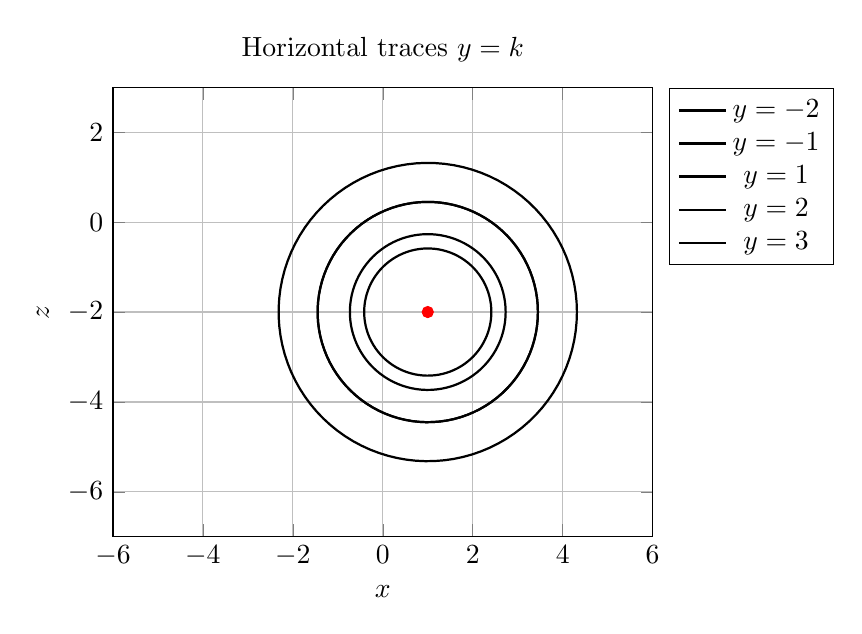
\begin{tikzpicture}
\begin{axis}[
    axis equal,
    xlabel=$x$,
    ylabel=$z$,
    title={Horizontal traces $y=k$},
    xmin=-6,xmax=6,
    ymin=-6,ymax=2,
    grid=both,
    legend pos=outer north east,
]
\pgfplotsinvokeforeach{-2,-1,1,2,3}{
\pgfmathsetmacro{\r}{sqrt(2+(#1-1)^2)}
\addplot[thick,domain=0:360,samples=100] ({1+\r*cos(x)},{-2+\r*sin(x)});
\addlegendentryexpanded{$y=#1$}
}
\addplot[only marks,mark=*,red] coordinates {(1,-2)};
\end{axis}
\end{tikzpicture}
\end{document}
